\section{Differential Algebraic Equations (DAE)}
\begin{figure}[H]
    \centering
    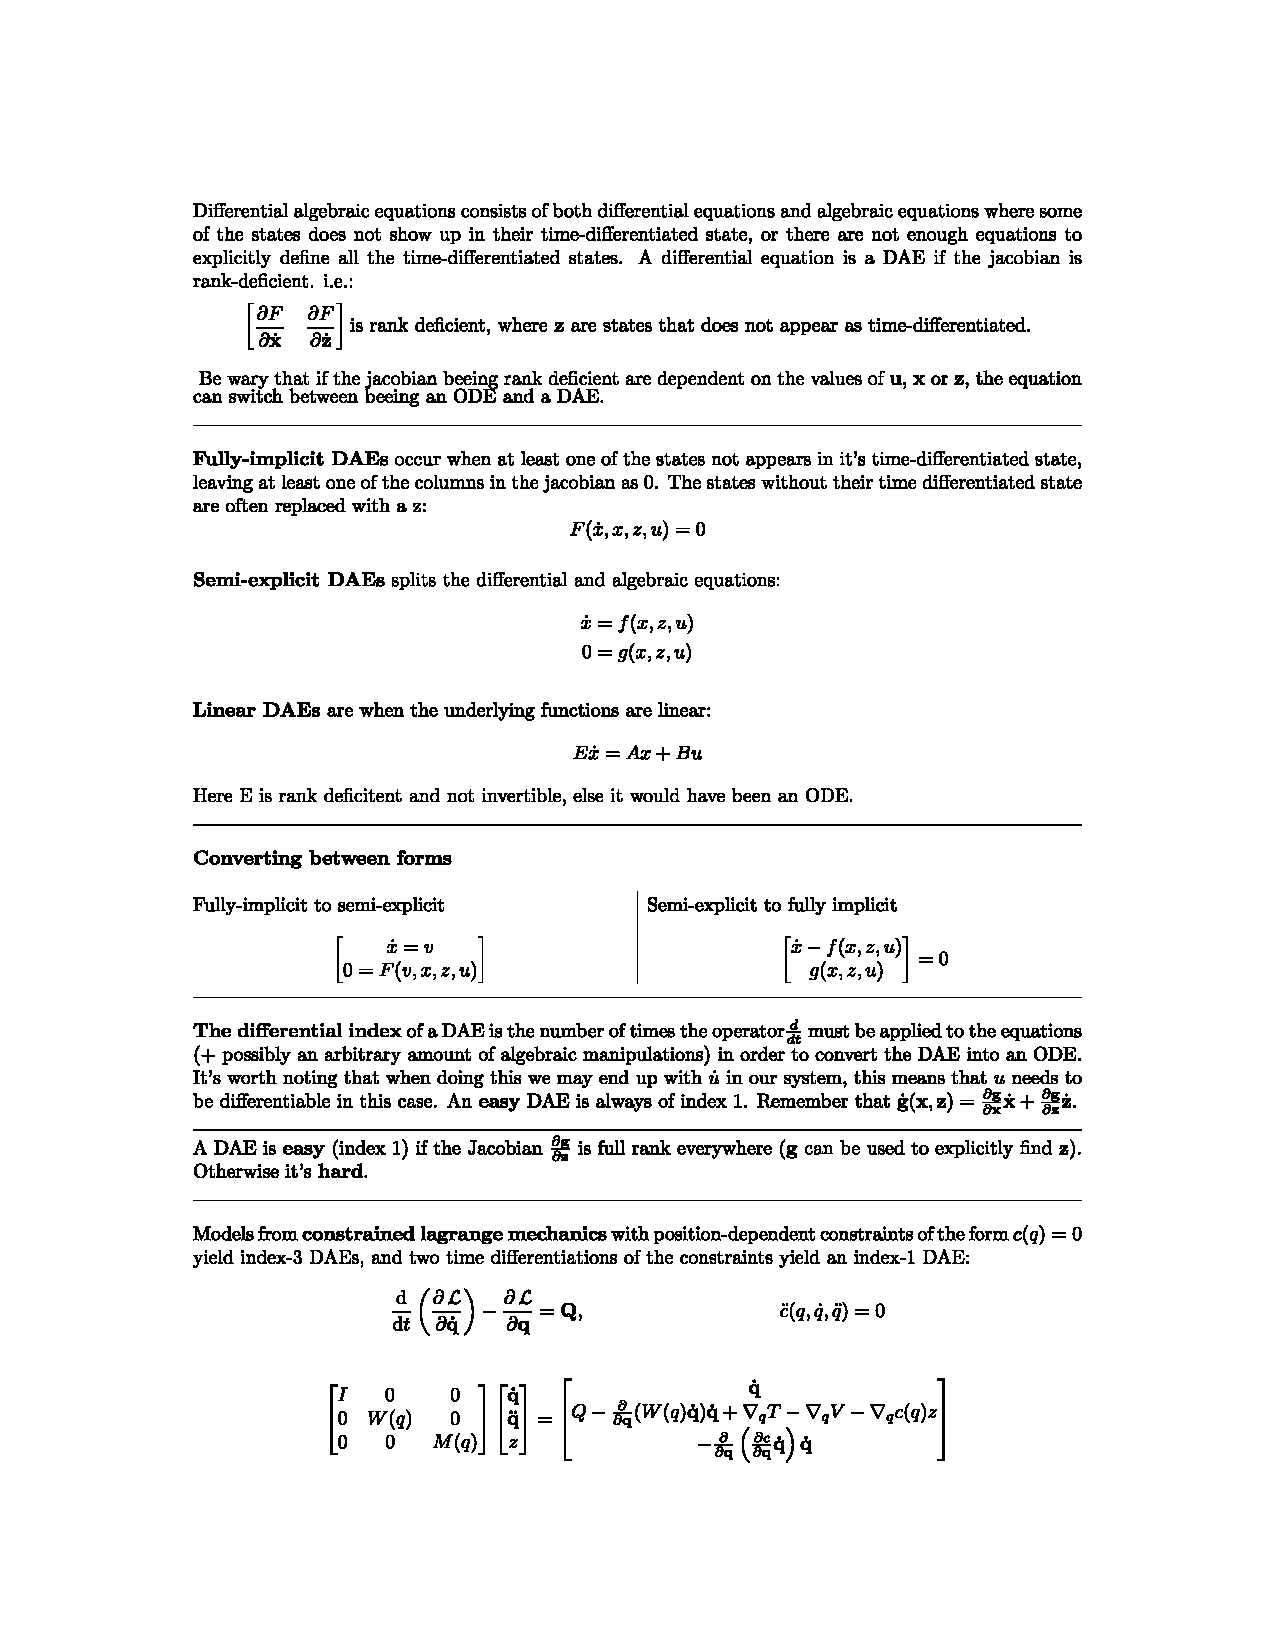
\includepdf[width=\linewidth]{figures/dae1.pdf}
\end{figure}
\newpage
\begin{figure}
    \centering
    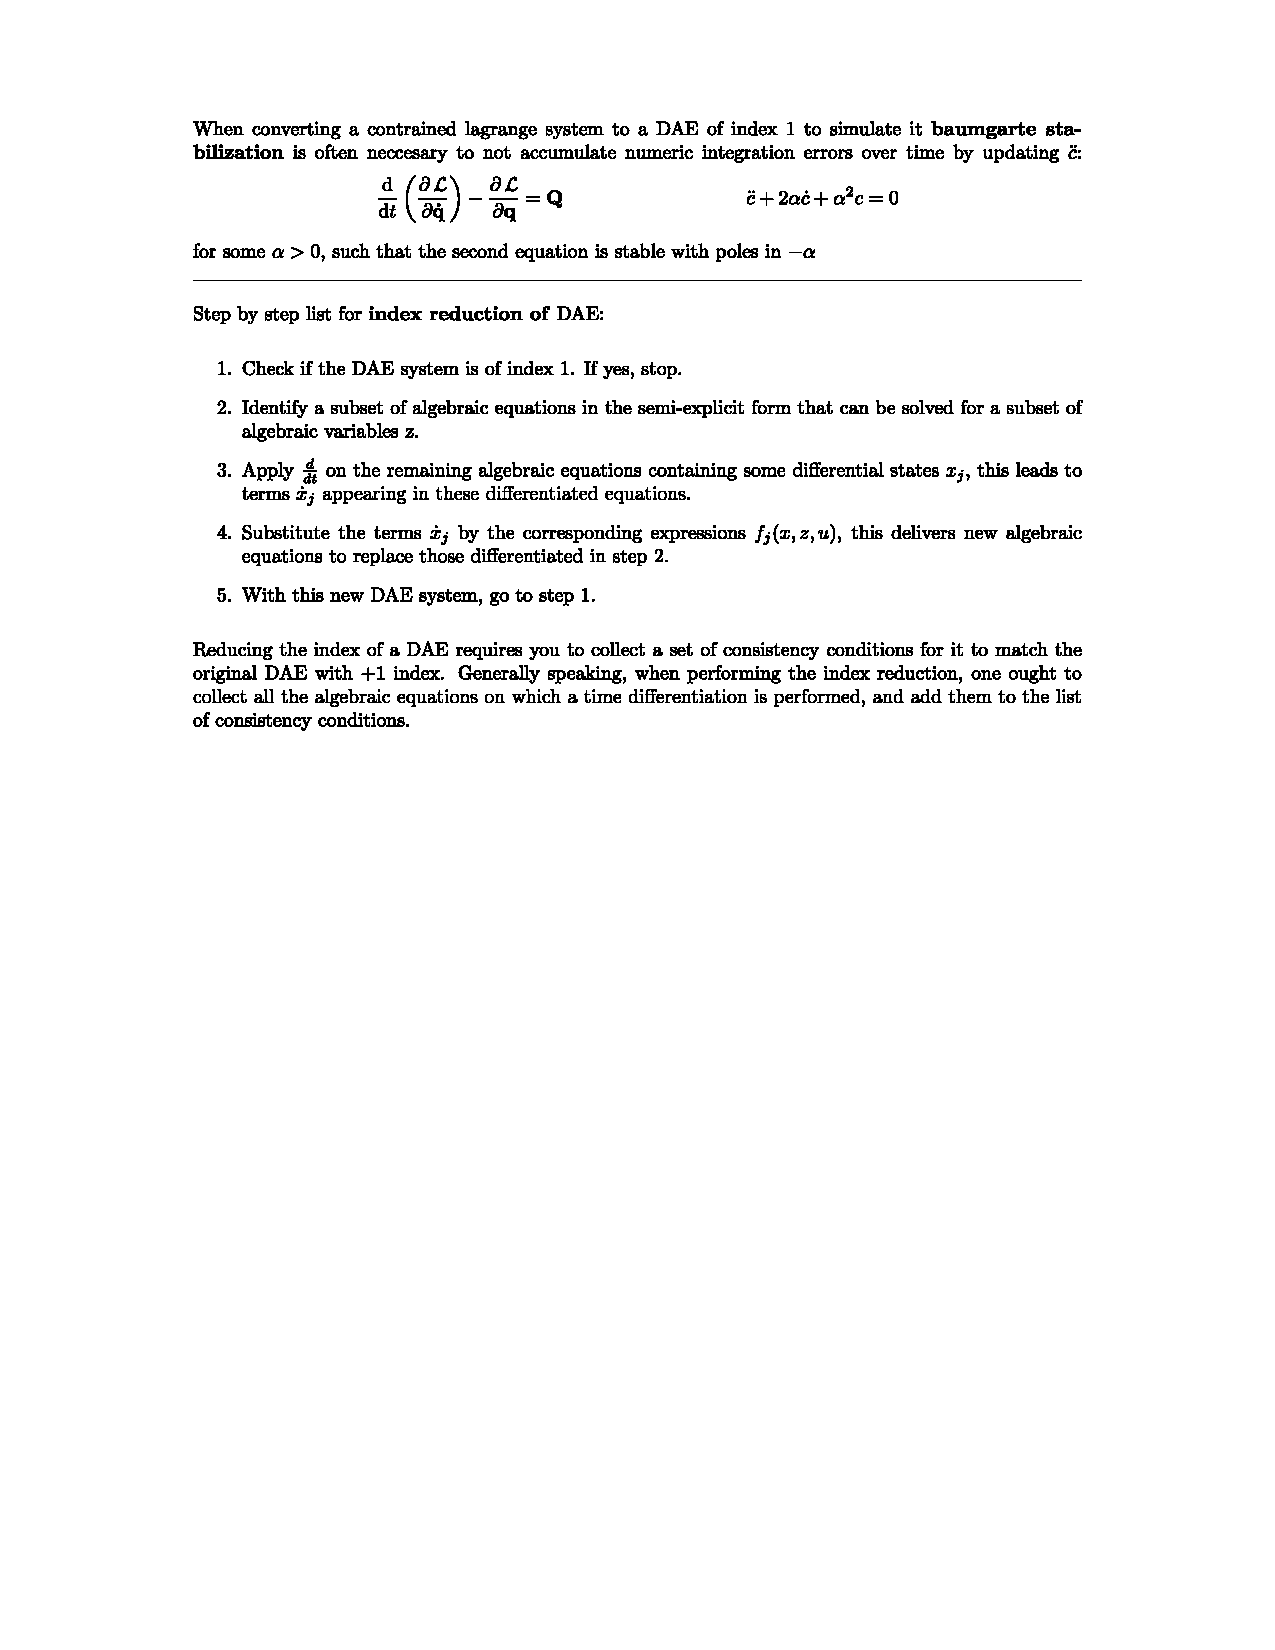
\includepdf[width=\linewidth]{figures/dae2.pdf}
\end{figure}
You rarely want to reduce to index 0, because the more you differentiate, the more information you lose/the bigger error you introduce.
The consistency conditions are simply the equations that are not differentiated. Your constraints if you are modelling with constrained lagrange for an example. 